
% Default to the notebook output style

    


% Inherit from the specified cell style.




    
\documentclass[11pt]{article}

    
    
    \usepackage[T1]{fontenc}
    % Nicer default font (+ math font) than Computer Modern for most use cases
    \usepackage{mathpazo}

    % Basic figure setup, for now with no caption control since it's done
    % automatically by Pandoc (which extracts ![](path) syntax from Markdown).
    \usepackage{graphicx}
    % We will generate all images so they have a width \maxwidth. This means
    % that they will get their normal width if they fit onto the page, but
    % are scaled down if they would overflow the margins.
    \makeatletter
    \def\maxwidth{\ifdim\Gin@nat@width>\linewidth\linewidth
    \else\Gin@nat@width\fi}
    \makeatother
    \let\Oldincludegraphics\includegraphics
    % Set max figure width to be 80% of text width, for now hardcoded.
    \renewcommand{\includegraphics}[1]{\Oldincludegraphics[width=.8\maxwidth]{#1}}
    % Ensure that by default, figures have no caption (until we provide a
    % proper Figure object with a Caption API and a way to capture that
    % in the conversion process - todo).
    \usepackage{caption}
    \DeclareCaptionLabelFormat{nolabel}{}
    \captionsetup{labelformat=nolabel}

    \usepackage{adjustbox} % Used to constrain images to a maximum size 
    \usepackage{xcolor} % Allow colors to be defined
    \usepackage{enumerate} % Needed for markdown enumerations to work
    \usepackage{geometry} % Used to adjust the document margins
    \usepackage{amsmath} % Equations
    \usepackage{amssymb} % Equations
    \usepackage{textcomp} % defines textquotesingle
    % Hack from http://tex.stackexchange.com/a/47451/13684:
    \AtBeginDocument{%
        \def\PYZsq{\textquotesingle}% Upright quotes in Pygmentized code
    }
    \usepackage{upquote} % Upright quotes for verbatim code
    \usepackage{eurosym} % defines \euro
    \usepackage[mathletters]{ucs} % Extended unicode (utf-8) support
    \usepackage[utf8x]{inputenc} % Allow utf-8 characters in the tex document
    \usepackage{fancyvrb} % verbatim replacement that allows latex
    \usepackage{grffile} % extends the file name processing of package graphics 
                         % to support a larger range 
    % The hyperref package gives us a pdf with properly built
    % internal navigation ('pdf bookmarks' for the table of contents,
    % internal cross-reference links, web links for URLs, etc.)
    \usepackage{hyperref}
    \usepackage{longtable} % longtable support required by pandoc >1.10
    \usepackage{booktabs}  % table support for pandoc > 1.12.2
    \usepackage[inline]{enumitem} % IRkernel/repr support (it uses the enumerate* environment)
    \usepackage[normalem]{ulem} % ulem is needed to support strikethroughs (\sout)
                                % normalem makes italics be italics, not underlines
    

    
    
    % Colors for the hyperref package
    \definecolor{urlcolor}{rgb}{0,.145,.698}
    \definecolor{linkcolor}{rgb}{.71,0.21,0.01}
    \definecolor{citecolor}{rgb}{.12,.54,.11}

    % ANSI colors
    \definecolor{ansi-black}{HTML}{3E424D}
    \definecolor{ansi-black-intense}{HTML}{282C36}
    \definecolor{ansi-red}{HTML}{E75C58}
    \definecolor{ansi-red-intense}{HTML}{B22B31}
    \definecolor{ansi-green}{HTML}{00A250}
    \definecolor{ansi-green-intense}{HTML}{007427}
    \definecolor{ansi-yellow}{HTML}{DDB62B}
    \definecolor{ansi-yellow-intense}{HTML}{B27D12}
    \definecolor{ansi-blue}{HTML}{208FFB}
    \definecolor{ansi-blue-intense}{HTML}{0065CA}
    \definecolor{ansi-magenta}{HTML}{D160C4}
    \definecolor{ansi-magenta-intense}{HTML}{A03196}
    \definecolor{ansi-cyan}{HTML}{60C6C8}
    \definecolor{ansi-cyan-intense}{HTML}{258F8F}
    \definecolor{ansi-white}{HTML}{C5C1B4}
    \definecolor{ansi-white-intense}{HTML}{A1A6B2}

    % commands and environments needed by pandoc snippets
    % extracted from the output of `pandoc -s`
    \providecommand{\tightlist}{%
      \setlength{\itemsep}{0pt}\setlength{\parskip}{0pt}}
    \DefineVerbatimEnvironment{Highlighting}{Verbatim}{commandchars=\\\{\}}
    % Add ',fontsize=\small' for more characters per line
    \newenvironment{Shaded}{}{}
    \newcommand{\KeywordTok}[1]{\textcolor[rgb]{0.00,0.44,0.13}{\textbf{{#1}}}}
    \newcommand{\DataTypeTok}[1]{\textcolor[rgb]{0.56,0.13,0.00}{{#1}}}
    \newcommand{\DecValTok}[1]{\textcolor[rgb]{0.25,0.63,0.44}{{#1}}}
    \newcommand{\BaseNTok}[1]{\textcolor[rgb]{0.25,0.63,0.44}{{#1}}}
    \newcommand{\FloatTok}[1]{\textcolor[rgb]{0.25,0.63,0.44}{{#1}}}
    \newcommand{\CharTok}[1]{\textcolor[rgb]{0.25,0.44,0.63}{{#1}}}
    \newcommand{\StringTok}[1]{\textcolor[rgb]{0.25,0.44,0.63}{{#1}}}
    \newcommand{\CommentTok}[1]{\textcolor[rgb]{0.38,0.63,0.69}{\textit{{#1}}}}
    \newcommand{\OtherTok}[1]{\textcolor[rgb]{0.00,0.44,0.13}{{#1}}}
    \newcommand{\AlertTok}[1]{\textcolor[rgb]{1.00,0.00,0.00}{\textbf{{#1}}}}
    \newcommand{\FunctionTok}[1]{\textcolor[rgb]{0.02,0.16,0.49}{{#1}}}
    \newcommand{\RegionMarkerTok}[1]{{#1}}
    \newcommand{\ErrorTok}[1]{\textcolor[rgb]{1.00,0.00,0.00}{\textbf{{#1}}}}
    \newcommand{\NormalTok}[1]{{#1}}
    
    % Additional commands for more recent versions of Pandoc
    \newcommand{\ConstantTok}[1]{\textcolor[rgb]{0.53,0.00,0.00}{{#1}}}
    \newcommand{\SpecialCharTok}[1]{\textcolor[rgb]{0.25,0.44,0.63}{{#1}}}
    \newcommand{\VerbatimStringTok}[1]{\textcolor[rgb]{0.25,0.44,0.63}{{#1}}}
    \newcommand{\SpecialStringTok}[1]{\textcolor[rgb]{0.73,0.40,0.53}{{#1}}}
    \newcommand{\ImportTok}[1]{{#1}}
    \newcommand{\DocumentationTok}[1]{\textcolor[rgb]{0.73,0.13,0.13}{\textit{{#1}}}}
    \newcommand{\AnnotationTok}[1]{\textcolor[rgb]{0.38,0.63,0.69}{\textbf{\textit{{#1}}}}}
    \newcommand{\CommentVarTok}[1]{\textcolor[rgb]{0.38,0.63,0.69}{\textbf{\textit{{#1}}}}}
    \newcommand{\VariableTok}[1]{\textcolor[rgb]{0.10,0.09,0.49}{{#1}}}
    \newcommand{\ControlFlowTok}[1]{\textcolor[rgb]{0.00,0.44,0.13}{\textbf{{#1}}}}
    \newcommand{\OperatorTok}[1]{\textcolor[rgb]{0.40,0.40,0.40}{{#1}}}
    \newcommand{\BuiltInTok}[1]{{#1}}
    \newcommand{\ExtensionTok}[1]{{#1}}
    \newcommand{\PreprocessorTok}[1]{\textcolor[rgb]{0.74,0.48,0.00}{{#1}}}
    \newcommand{\AttributeTok}[1]{\textcolor[rgb]{0.49,0.56,0.16}{{#1}}}
    \newcommand{\InformationTok}[1]{\textcolor[rgb]{0.38,0.63,0.69}{\textbf{\textit{{#1}}}}}
    \newcommand{\WarningTok}[1]{\textcolor[rgb]{0.38,0.63,0.69}{\textbf{\textit{{#1}}}}}
    
    
    % Define a nice break command that doesn't care if a line doesn't already
    % exist.
    \def\br{\hspace*{\fill} \\* }
    % Math Jax compatability definitions
    \def\gt{>}
    \def\lt{<}
    % Document parameters
    \title{Quantum Computing Basics}
    
    
    

    % Pygments definitions
    
\makeatletter
\def\PY@reset{\let\PY@it=\relax \let\PY@bf=\relax%
    \let\PY@ul=\relax \let\PY@tc=\relax%
    \let\PY@bc=\relax \let\PY@ff=\relax}
\def\PY@tok#1{\csname PY@tok@#1\endcsname}
\def\PY@toks#1+{\ifx\relax#1\empty\else%
    \PY@tok{#1}\expandafter\PY@toks\fi}
\def\PY@do#1{\PY@bc{\PY@tc{\PY@ul{%
    \PY@it{\PY@bf{\PY@ff{#1}}}}}}}
\def\PY#1#2{\PY@reset\PY@toks#1+\relax+\PY@do{#2}}

\expandafter\def\csname PY@tok@w\endcsname{\def\PY@tc##1{\textcolor[rgb]{0.73,0.73,0.73}{##1}}}
\expandafter\def\csname PY@tok@c\endcsname{\let\PY@it=\textit\def\PY@tc##1{\textcolor[rgb]{0.25,0.50,0.50}{##1}}}
\expandafter\def\csname PY@tok@cp\endcsname{\def\PY@tc##1{\textcolor[rgb]{0.74,0.48,0.00}{##1}}}
\expandafter\def\csname PY@tok@k\endcsname{\let\PY@bf=\textbf\def\PY@tc##1{\textcolor[rgb]{0.00,0.50,0.00}{##1}}}
\expandafter\def\csname PY@tok@kp\endcsname{\def\PY@tc##1{\textcolor[rgb]{0.00,0.50,0.00}{##1}}}
\expandafter\def\csname PY@tok@kt\endcsname{\def\PY@tc##1{\textcolor[rgb]{0.69,0.00,0.25}{##1}}}
\expandafter\def\csname PY@tok@o\endcsname{\def\PY@tc##1{\textcolor[rgb]{0.40,0.40,0.40}{##1}}}
\expandafter\def\csname PY@tok@ow\endcsname{\let\PY@bf=\textbf\def\PY@tc##1{\textcolor[rgb]{0.67,0.13,1.00}{##1}}}
\expandafter\def\csname PY@tok@nb\endcsname{\def\PY@tc##1{\textcolor[rgb]{0.00,0.50,0.00}{##1}}}
\expandafter\def\csname PY@tok@nf\endcsname{\def\PY@tc##1{\textcolor[rgb]{0.00,0.00,1.00}{##1}}}
\expandafter\def\csname PY@tok@nc\endcsname{\let\PY@bf=\textbf\def\PY@tc##1{\textcolor[rgb]{0.00,0.00,1.00}{##1}}}
\expandafter\def\csname PY@tok@nn\endcsname{\let\PY@bf=\textbf\def\PY@tc##1{\textcolor[rgb]{0.00,0.00,1.00}{##1}}}
\expandafter\def\csname PY@tok@ne\endcsname{\let\PY@bf=\textbf\def\PY@tc##1{\textcolor[rgb]{0.82,0.25,0.23}{##1}}}
\expandafter\def\csname PY@tok@nv\endcsname{\def\PY@tc##1{\textcolor[rgb]{0.10,0.09,0.49}{##1}}}
\expandafter\def\csname PY@tok@no\endcsname{\def\PY@tc##1{\textcolor[rgb]{0.53,0.00,0.00}{##1}}}
\expandafter\def\csname PY@tok@nl\endcsname{\def\PY@tc##1{\textcolor[rgb]{0.63,0.63,0.00}{##1}}}
\expandafter\def\csname PY@tok@ni\endcsname{\let\PY@bf=\textbf\def\PY@tc##1{\textcolor[rgb]{0.60,0.60,0.60}{##1}}}
\expandafter\def\csname PY@tok@na\endcsname{\def\PY@tc##1{\textcolor[rgb]{0.49,0.56,0.16}{##1}}}
\expandafter\def\csname PY@tok@nt\endcsname{\let\PY@bf=\textbf\def\PY@tc##1{\textcolor[rgb]{0.00,0.50,0.00}{##1}}}
\expandafter\def\csname PY@tok@nd\endcsname{\def\PY@tc##1{\textcolor[rgb]{0.67,0.13,1.00}{##1}}}
\expandafter\def\csname PY@tok@s\endcsname{\def\PY@tc##1{\textcolor[rgb]{0.73,0.13,0.13}{##1}}}
\expandafter\def\csname PY@tok@sd\endcsname{\let\PY@it=\textit\def\PY@tc##1{\textcolor[rgb]{0.73,0.13,0.13}{##1}}}
\expandafter\def\csname PY@tok@si\endcsname{\let\PY@bf=\textbf\def\PY@tc##1{\textcolor[rgb]{0.73,0.40,0.53}{##1}}}
\expandafter\def\csname PY@tok@se\endcsname{\let\PY@bf=\textbf\def\PY@tc##1{\textcolor[rgb]{0.73,0.40,0.13}{##1}}}
\expandafter\def\csname PY@tok@sr\endcsname{\def\PY@tc##1{\textcolor[rgb]{0.73,0.40,0.53}{##1}}}
\expandafter\def\csname PY@tok@ss\endcsname{\def\PY@tc##1{\textcolor[rgb]{0.10,0.09,0.49}{##1}}}
\expandafter\def\csname PY@tok@sx\endcsname{\def\PY@tc##1{\textcolor[rgb]{0.00,0.50,0.00}{##1}}}
\expandafter\def\csname PY@tok@m\endcsname{\def\PY@tc##1{\textcolor[rgb]{0.40,0.40,0.40}{##1}}}
\expandafter\def\csname PY@tok@gh\endcsname{\let\PY@bf=\textbf\def\PY@tc##1{\textcolor[rgb]{0.00,0.00,0.50}{##1}}}
\expandafter\def\csname PY@tok@gu\endcsname{\let\PY@bf=\textbf\def\PY@tc##1{\textcolor[rgb]{0.50,0.00,0.50}{##1}}}
\expandafter\def\csname PY@tok@gd\endcsname{\def\PY@tc##1{\textcolor[rgb]{0.63,0.00,0.00}{##1}}}
\expandafter\def\csname PY@tok@gi\endcsname{\def\PY@tc##1{\textcolor[rgb]{0.00,0.63,0.00}{##1}}}
\expandafter\def\csname PY@tok@gr\endcsname{\def\PY@tc##1{\textcolor[rgb]{1.00,0.00,0.00}{##1}}}
\expandafter\def\csname PY@tok@ge\endcsname{\let\PY@it=\textit}
\expandafter\def\csname PY@tok@gs\endcsname{\let\PY@bf=\textbf}
\expandafter\def\csname PY@tok@gp\endcsname{\let\PY@bf=\textbf\def\PY@tc##1{\textcolor[rgb]{0.00,0.00,0.50}{##1}}}
\expandafter\def\csname PY@tok@go\endcsname{\def\PY@tc##1{\textcolor[rgb]{0.53,0.53,0.53}{##1}}}
\expandafter\def\csname PY@tok@gt\endcsname{\def\PY@tc##1{\textcolor[rgb]{0.00,0.27,0.87}{##1}}}
\expandafter\def\csname PY@tok@err\endcsname{\def\PY@bc##1{\setlength{\fboxsep}{0pt}\fcolorbox[rgb]{1.00,0.00,0.00}{1,1,1}{\strut ##1}}}
\expandafter\def\csname PY@tok@kc\endcsname{\let\PY@bf=\textbf\def\PY@tc##1{\textcolor[rgb]{0.00,0.50,0.00}{##1}}}
\expandafter\def\csname PY@tok@kd\endcsname{\let\PY@bf=\textbf\def\PY@tc##1{\textcolor[rgb]{0.00,0.50,0.00}{##1}}}
\expandafter\def\csname PY@tok@kn\endcsname{\let\PY@bf=\textbf\def\PY@tc##1{\textcolor[rgb]{0.00,0.50,0.00}{##1}}}
\expandafter\def\csname PY@tok@kr\endcsname{\let\PY@bf=\textbf\def\PY@tc##1{\textcolor[rgb]{0.00,0.50,0.00}{##1}}}
\expandafter\def\csname PY@tok@bp\endcsname{\def\PY@tc##1{\textcolor[rgb]{0.00,0.50,0.00}{##1}}}
\expandafter\def\csname PY@tok@fm\endcsname{\def\PY@tc##1{\textcolor[rgb]{0.00,0.00,1.00}{##1}}}
\expandafter\def\csname PY@tok@vc\endcsname{\def\PY@tc##1{\textcolor[rgb]{0.10,0.09,0.49}{##1}}}
\expandafter\def\csname PY@tok@vg\endcsname{\def\PY@tc##1{\textcolor[rgb]{0.10,0.09,0.49}{##1}}}
\expandafter\def\csname PY@tok@vi\endcsname{\def\PY@tc##1{\textcolor[rgb]{0.10,0.09,0.49}{##1}}}
\expandafter\def\csname PY@tok@vm\endcsname{\def\PY@tc##1{\textcolor[rgb]{0.10,0.09,0.49}{##1}}}
\expandafter\def\csname PY@tok@sa\endcsname{\def\PY@tc##1{\textcolor[rgb]{0.73,0.13,0.13}{##1}}}
\expandafter\def\csname PY@tok@sb\endcsname{\def\PY@tc##1{\textcolor[rgb]{0.73,0.13,0.13}{##1}}}
\expandafter\def\csname PY@tok@sc\endcsname{\def\PY@tc##1{\textcolor[rgb]{0.73,0.13,0.13}{##1}}}
\expandafter\def\csname PY@tok@dl\endcsname{\def\PY@tc##1{\textcolor[rgb]{0.73,0.13,0.13}{##1}}}
\expandafter\def\csname PY@tok@s2\endcsname{\def\PY@tc##1{\textcolor[rgb]{0.73,0.13,0.13}{##1}}}
\expandafter\def\csname PY@tok@sh\endcsname{\def\PY@tc##1{\textcolor[rgb]{0.73,0.13,0.13}{##1}}}
\expandafter\def\csname PY@tok@s1\endcsname{\def\PY@tc##1{\textcolor[rgb]{0.73,0.13,0.13}{##1}}}
\expandafter\def\csname PY@tok@mb\endcsname{\def\PY@tc##1{\textcolor[rgb]{0.40,0.40,0.40}{##1}}}
\expandafter\def\csname PY@tok@mf\endcsname{\def\PY@tc##1{\textcolor[rgb]{0.40,0.40,0.40}{##1}}}
\expandafter\def\csname PY@tok@mh\endcsname{\def\PY@tc##1{\textcolor[rgb]{0.40,0.40,0.40}{##1}}}
\expandafter\def\csname PY@tok@mi\endcsname{\def\PY@tc##1{\textcolor[rgb]{0.40,0.40,0.40}{##1}}}
\expandafter\def\csname PY@tok@il\endcsname{\def\PY@tc##1{\textcolor[rgb]{0.40,0.40,0.40}{##1}}}
\expandafter\def\csname PY@tok@mo\endcsname{\def\PY@tc##1{\textcolor[rgb]{0.40,0.40,0.40}{##1}}}
\expandafter\def\csname PY@tok@ch\endcsname{\let\PY@it=\textit\def\PY@tc##1{\textcolor[rgb]{0.25,0.50,0.50}{##1}}}
\expandafter\def\csname PY@tok@cm\endcsname{\let\PY@it=\textit\def\PY@tc##1{\textcolor[rgb]{0.25,0.50,0.50}{##1}}}
\expandafter\def\csname PY@tok@cpf\endcsname{\let\PY@it=\textit\def\PY@tc##1{\textcolor[rgb]{0.25,0.50,0.50}{##1}}}
\expandafter\def\csname PY@tok@c1\endcsname{\let\PY@it=\textit\def\PY@tc##1{\textcolor[rgb]{0.25,0.50,0.50}{##1}}}
\expandafter\def\csname PY@tok@cs\endcsname{\let\PY@it=\textit\def\PY@tc##1{\textcolor[rgb]{0.25,0.50,0.50}{##1}}}

\def\PYZbs{\char`\\}
\def\PYZus{\char`\_}
\def\PYZob{\char`\{}
\def\PYZcb{\char`\}}
\def\PYZca{\char`\^}
\def\PYZam{\char`\&}
\def\PYZlt{\char`\<}
\def\PYZgt{\char`\>}
\def\PYZsh{\char`\#}
\def\PYZpc{\char`\%}
\def\PYZdl{\char`\$}
\def\PYZhy{\char`\-}
\def\PYZsq{\char`\'}
\def\PYZdq{\char`\"}
\def\PYZti{\char`\~}
% for compatibility with earlier versions
\def\PYZat{@}
\def\PYZlb{[}
\def\PYZrb{]}
\makeatother


    % Exact colors from NB
    \definecolor{incolor}{rgb}{0.0, 0.0, 0.5}
    \definecolor{outcolor}{rgb}{0.545, 0.0, 0.0}



    
    % Prevent overflowing lines due to hard-to-break entities
    \sloppy 
    % Setup hyperref package
    \hypersetup{
      breaklinks=true,  % so long urls are correctly broken across lines
      colorlinks=true,
      urlcolor=urlcolor,
      linkcolor=linkcolor,
      citecolor=citecolor,
      }
    % Slightly bigger margins than the latex defaults
    
    \geometry{verbose,tmargin=1in,bmargin=1in,lmargin=1in,rmargin=1in}
    
    

    \begin{document}
    
    
    \maketitle
    
    

    
    \section{A Breif Introduction to Quantum
Mechanics}\label{a-breif-introduction-to-quantum-mechanics}

    Quantum mechanics studies the smallest parts of our universe. One main
difference between the quantum mechanical world, and the world we
interact with daily, is that quantum particles behave probabilistically.
That is, where a classical object will always follow the same
interactions, quantum particles behave differently each time, with their
behavior defined by probability density functions. A particles
probability density function is given by its \emph{wavefunction},
\(\psi(x)\), where \(|\psi(x)|^2\) (magnitude squared) is the
probability to find that particle at position \(x\).

What does it mean to define a particle's position by a continuous
function? This is where quantum mechanics requires a new method of
thinking. Normally when we think of an object's position, it can be
defined in terms of \((x, y, z)\) coordinates, and exists only in that
location. Quantum particles, however, somewhat "exist" in \emph{all}
locations until measured. Once measured, the continuous wavefunction
will collapse into a single point, defining the location of the
particle.

For example, if a particle has a wave function defined by a sine
function on the interval \([0, \pi]\), the PDF will look like:

\begin{figure}
\centering
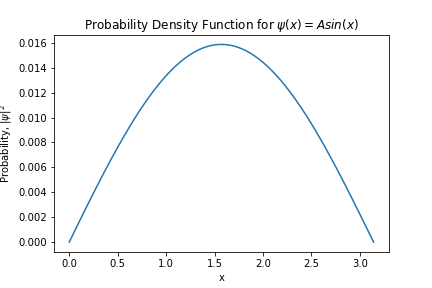
\includegraphics{images/sin_pdf.png}
\caption{}
\end{figure}

    Notice that the function has some normalization constant out front. This
is required as the total probability for existence must be equal to one.
Mathematically, the normalization constant can be found by integrating
the entire PDF which is equal to one, then solving for the constant;
however, that goes slightly beyond the scope of quantum computing
basics.

This wavefunction suggests that the \emph{most likely} location to
measure our particle is in the middle at \(\frac{\pi}{2}\). However, if
we were to measure a series of particles that had this wavefunction, not
all would be located at \(\frac{\pi}{2}\), which is the most important
point of this example. The location of particles are probabilistically
defined by their wavefunctions, and are unknown until measured. This
phenomenon is the beginning of what gives quantum processors their
advantages over classical computers and will become more apparent in
future sections.

    \subsubsection{Dirac Notation}\label{dirac-notation}

    Before continuing into quantum mechanics, it is important to establish a
different style for representing linear algebra. Dirac notation, also
known as Bra-Ket notation, allows us to easily represent quantum states.
Bra-ket notation uses two new vector representations, bras and kets,
which are equivalent to row vectors and column vectors, respectively.
Bras are represented as \[\langle a |\] and kets by \[| b \rangle\]

We define some general bras and kets, each with two elements, for
example purposes:

\[\langle a | = \begin{pmatrix} a_1 \ a_2 \end{pmatrix}\]

\[| b \rangle = \begin{pmatrix} b_1 \\ b_2 \end{pmatrix}\]

Like normal vectors, bras and kets can be scaled

\[n\langle a | = \begin{pmatrix} na_1 \ na_2 \end{pmatrix}\]

\[n| b \rangle = \begin{pmatrix} nb_1 \\ nb_2 \end{pmatrix}\]

Bras can be added to bras, and kets can be added to kets

\[ | b \rangle + | c \rangle =  \begin{pmatrix} b_1 \\ b_2 \end{pmatrix} + \begin{pmatrix} c_1 \\ c_2 \end{pmatrix} = \begin{pmatrix} b_1 + c_1 \\ b_2 + c_2 \end{pmatrix}\]

A bra can be transformed into a ket and vice versa by taking the
conjugate transpose, or dagger operator of the state:

\[\langle a |^{*T} = \langle a |^\dagger = \begin{pmatrix} a_1 \ a_2 \end{pmatrix}^\dagger = \begin{pmatrix} a_1^* \\ a_2^* \end{pmatrix} = | a \rangle\]

And a normal linear algebra dot product is represented by

\[\langle a | b \rangle = \begin{pmatrix} a_1 \ a_2 \end{pmatrix} \cdot \begin{pmatrix} b_1 \\ b_2 \end{pmatrix} = a_1b_1 + a_2b_2\]

which is referred to as the \emph{inner product}. Reversing the ordering
of thse bra/ket results in matrix multiplication, also known as the
\emph{outer product}.

\[ | b \rangle \langle a | = \begin{pmatrix} b_1 \\ b_2 \end{pmatrix} \begin{pmatrix} a_1 \ a_2 \end{pmatrix}  = \begin{pmatrix} b_1a_1 & b_1a_2 \\ b_2a_1 & b_2a_2 \end{pmatrix} \]

    \subsubsection{Basis Vectors and
Superposition}\label{basis-vectors-and-superposition}

    Bras and kets are used to define the \textbf{basis vectors} which will
be incredibly important going forwards. In the Z basis, these are
defined as

\[|0\rangle \ = \ \begin{pmatrix} 1 \\ 0 \end{pmatrix} \ \ \ \ \ \ |1\rangle \ = \ \begin{pmatrix} 0 \\ 1 \end{pmatrix}\]

These are the most fundamental vectors for our purposes, as a particle
in the \(|0\rangle\) state will have an output measurement of 0, and a
particle in the state \(|1\rangle\) state will have an output
measurement of 1, \emph{when taking a z measurement}.

It is possible for a particle to be in a \emph{linear combination} of
states. For example, a particle might be in the general state
\[|\psi\rangle = \alpha|0\rangle + \beta|1\rangle\] where \(\alpha\) and
\(\beta\) are constants. Quantum states must also always be normalized
meaning \(|\alpha|^2 + |\beta|^2 = 1\). The particle existing in this
linear combination of states is referred to as \emph{superposition}.
When measuring a qubit, the resulting output will either be a 0 or a 1,
meaning that our superposition state is not directly observable. When
measuring the state \(|\psi\rangle\), the probability of meauring a 0
will be \(|\alpha|^2\), and the probability of measusing 1 will be
\(|\beta|^2\).

Let us solve for a state which has equal probabilities for the outcome
of a z measurement. Equal probabilities means
\(|\alpha|^2 = |\beta|^2\), and using our normalization condition we can
solve for the constants.

\[|\alpha|^2 + |\beta|^2 = 1\]

\[2|\alpha|^2 = 1\]

\[\alpha = \frac{1}{\sqrt{2}}\]

\[\implies |\psi\rangle = \frac{1}{\sqrt{2}}(|0\rangle + |1\rangle)\]

We will see that measuring a particle in this state will result in equal
measurements of 0 and 1. The state we just produced is considered the
\textbf{x basis}, with the state symbols given as

\[|+\rangle = \frac{1}{\sqrt{2}}(|0\rangle + |1\rangle)\]

and

\[|-\rangle = \frac{1}{\sqrt{2}}(|0\rangle - |1\rangle)\]

The third basis, which is the \textbf{y basis}, is defined with complex
numbers, as follows

\[|\circlearrowright\rangle = \frac{ | 0 \rangle + i | 1 \rangle}{\sqrt{2}}\]

\[|\circlearrowleft\rangle = \frac{ | 0 \rangle -i | 1 \rangle}{\sqrt{2}}\]

    \subsubsection{Classical Bits versus Quantum Bits
(Qubits)}\label{classical-bits-versus-quantum-bits-qubits}

    The quantum mechanical particles described above are the base unit of
quantum information used in a quantum computer. Where in classical
computing the base unit is called a \emph{bit}, in quantum computing
they are called quantum bits, or \emph{qubits}. A single qubit can be in
the states described above, and it is the physical entity that we
manipulate and measure.

A classical bit is straightforward and easy to define. A bit either
takes the value of a 0 or a 1. The classical bit is in a single state at
any given time, and any measurement will simply result in that state,
which is intuitive. As described above, the qubit can be in 0 or 1 like
the classical bit, but it can also be in any state between 0 or 1. This
is much easier visualized on the \textbf{Bloch Sphere}, which is the
unit sphere representing the possible linear combinations between the x,
y, and z basis. The following figure shows the Block sphere, with a
vector representing the \(|0\rangle\) state.

\begin{figure}
\centering
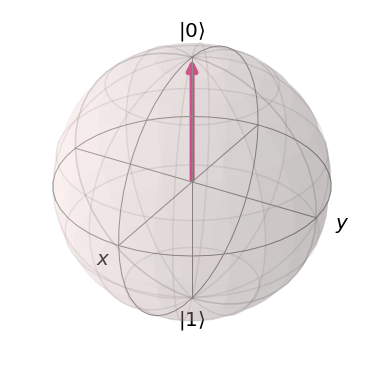
\includegraphics{images/bloch_0.png}
\caption{}
\end{figure}

    The \(|+\rangle\) state points purely along the x axis, which is halfway
between \(|0\rangle\) and \(|1\rangle\).

\begin{figure}
\centering
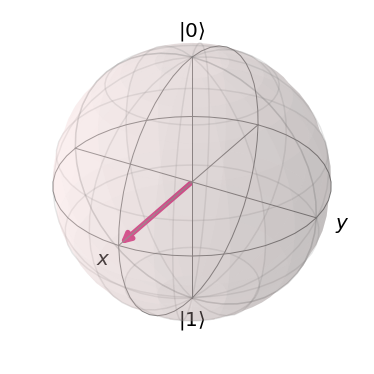
\includegraphics{images/bloch_+.png}
\caption{}
\end{figure}

And the \(|\circlearrowright\rangle\) state is along the y axis.

\begin{figure}
\centering
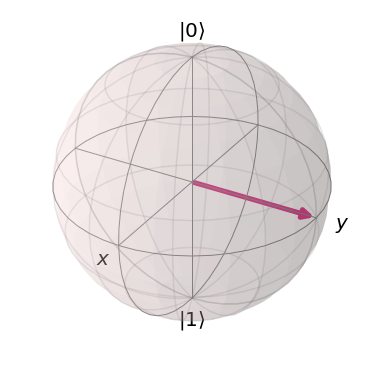
\includegraphics{images/bloch_y.png}
\caption{}
\end{figure}

    Along with the three sets of basis vectors, measurements are made for a
single base. The default measurement used in Qiskit measures the z
component of a state. When a particle is measured once and reveals an
outputs state, further measurements on that particle without any other
state changes will result in the same output. For example, if the
\(|+\rangle\) state was measured, and the outcome was 1, performing more
measurements would \emph{always} result in 1. However, after measuring
in the z base, the particles x and y measurements reset back to 50/50.
We will see how to manipulate the qubit to measure in the x and y basis
in the future, but it is important to note that the particle can only be
in one deterministic state at a time.

    \subsubsection{Manipulating Qubits}\label{manipulating-qubits}

    When qubits are initialized, they are put into the \(|0\rangle\) state.
In order the change a qubit's state, we use quantum gates. Quantum gates
have matrix representations, and typically perform rotations of the
vector around the Block sphere. The output state is given from the
matrix multiplication of the gate and the input state. We will start
with the simplest gates, known as the Paulis: \(X, Y\) and \(Z\). These
gates have the following matrix representations:

\[
X= \begin{pmatrix} 0&1 \\\\ 1&0 \end{pmatrix}\\\\
Y= \begin{pmatrix} 0&-i \\\\ i&0 \end{pmatrix}\\\\
Z= \begin{pmatrix} 1&0 \\\\ 0&-1 \end{pmatrix}
\]

We will look at an example of applying the \(X\) gate to the
\(|0\rangle\) state:

\[X |0\rangle = |1\rangle = \begin{pmatrix} 0&1 \\\\ 1&0 \end{pmatrix} \begin{pmatrix} 1 \\ 0 \end{pmatrix} = \begin{pmatrix} 0 \\ 1 \end{pmatrix} = |1\rangle\]

This takes a 0 input state and transforms it to a 1. Other transitions
are

\[
Z |+\rangle = |-\rangle, \\\\ Z |-\rangle = |+\rangle.
\]

\[
Y |0\rangle = i|1\rangle, \\\\ Y |1\rangle = -i|0\rangle.
\]

These are just a couple examples of how qubits can be manipulated. The
following sections will cover the various gates and their implementation
in Qiskit.

    \subsubsection{Quantum Circuits}\label{quantum-circuits}

    A quantum circuit represents the control flow that happens in a quantum
processor, defining the stages that gates are applied and when
measurements are taken. The following image is an example of a quantum
circuit. Two qubits are represented by \(q_0\) and \(q_1\). \(q_0\),
which is initially loaded as state \(|0\rangle\), as the Pauli \(X\)
gate applied. Then between the barriers (which are not physical, just
for the output diagram) both qubits are manipulated with another gate
(which will be discussed), and finally are measured into control qubits.

    

    The Python code for generating a circuit without any gates is as
follows:

    \begin{Verbatim}[commandchars=\\\{\}]
{\color{incolor}In [{\color{incolor}1}]:} \PY{k+kn}{from} \PY{n+nn}{qiskit} \PY{k}{import} \PY{o}{*}
        \PY{k+kn}{from} \PY{n+nn}{qiskit}\PY{n+nn}{.}\PY{n+nn}{visualization} \PY{k}{import} \PY{n}{plot\PYZus{}histogram}\PY{p}{,} \PY{n}{plot\PYZus{}bloch\PYZus{}vector}
\end{Verbatim}


    \begin{Verbatim}[commandchars=\\\{\}]
{\color{incolor}In [{\color{incolor}2}]:} \PY{n}{n\PYZus{}q} \PY{o}{=} \PY{l+m+mi}{2}  \PY{c+c1}{\PYZsh{} number of qubits}
        \PY{n}{n\PYZus{}b} \PY{o}{=} \PY{l+m+mi}{2}  \PY{c+c1}{\PYZsh{} number of output bits}
        \PY{n}{qc} \PY{o}{=} \PY{n}{QuantumCircuit}\PY{p}{(}\PY{n}{n\PYZus{}q}\PY{p}{,} \PY{n}{n\PYZus{}b}\PY{p}{)}
        \PY{n}{qc}\PY{o}{.}\PY{n}{draw}\PY{p}{(}\PY{n}{output}\PY{o}{=}\PY{l+s+s1}{\PYZsq{}}\PY{l+s+s1}{mpl}\PY{l+s+s1}{\PYZsq{}}\PY{p}{)}
\end{Verbatim}

\texttt{\color{outcolor}Out[{\color{outcolor}2}]:}
    
    \begin{center}
    \adjustimage{max size={0.9\linewidth}{0.9\paperheight}}{output_18_0.png}
    \end{center}
    { \hspace*{\fill} \\}
    

    Adding in some measurement gates

    \begin{Verbatim}[commandchars=\\\{\}]
{\color{incolor}In [{\color{incolor}3}]:} \PY{n}{qc}\PY{o}{.}\PY{n}{measure}\PY{p}{(}\PY{l+m+mi}{0}\PY{p}{,} \PY{l+m+mi}{0}\PY{p}{)}
        \PY{n}{qc}\PY{o}{.}\PY{n}{measure}\PY{p}{(}\PY{l+m+mi}{1}\PY{p}{,} \PY{l+m+mi}{1}\PY{p}{)}
        \PY{n}{qc}\PY{o}{.}\PY{n}{draw}\PY{p}{(}\PY{n}{output}\PY{o}{=}\PY{l+s+s1}{\PYZsq{}}\PY{l+s+s1}{mpl}\PY{l+s+s1}{\PYZsq{}}\PY{p}{)}
\end{Verbatim}

\texttt{\color{outcolor}Out[{\color{outcolor}3}]:}
    
    \begin{center}
    \adjustimage{max size={0.9\linewidth}{0.9\paperheight}}{output_20_0.png}
    \end{center}
    { \hspace*{\fill} \\}
    

    And running the program on a simulator, where we expect to see 0 as the
output state for both qubits

    \begin{Verbatim}[commandchars=\\\{\}]
{\color{incolor}In [{\color{incolor}4}]:} \PY{n}{counts} \PY{o}{=} \PY{n}{execute}\PY{p}{(}\PY{n}{qc}\PY{p}{,} \PY{n}{Aer}\PY{o}{.}\PY{n}{get\PYZus{}backend}\PY{p}{(}\PY{l+s+s1}{\PYZsq{}}\PY{l+s+s1}{qasm\PYZus{}simulator}\PY{l+s+s1}{\PYZsq{}}\PY{p}{)}\PY{p}{)}\PY{o}{.}\PY{n}{result}\PY{p}{(}\PY{p}{)}\PY{o}{.}\PY{n}{get\PYZus{}counts}\PY{p}{(}\PY{p}{)}
        \PY{n}{plot\PYZus{}histogram}\PY{p}{(}\PY{n}{counts}\PY{p}{)}
\end{Verbatim}

\texttt{\color{outcolor}Out[{\color{outcolor}4}]:}
    
    \begin{center}
    \adjustimage{max size={0.9\linewidth}{0.9\paperheight}}{output_22_0.png}
    \end{center}
    { \hspace*{\fill} \\}
    

    The output is stored as a 2 bit binary string, corresponding to each
qubit output state. We see a 100\% rate of measure 0 on both qubits
because we did nothing with the circuit. If we were to add the Pauli
\(X\) gate to \(q_0\), let's see what happens.

    \begin{Verbatim}[commandchars=\\\{\}]
{\color{incolor}In [{\color{incolor}5}]:} \PY{c+c1}{\PYZsh{} reinitialize our circuit to add the X gate partway through}
        \PY{n}{qc} \PY{o}{=} \PY{n}{QuantumCircuit}\PY{p}{(}\PY{n}{n\PYZus{}q}\PY{p}{,} \PY{n}{n\PYZus{}b}\PY{p}{)}
        \PY{n}{qc}\PY{o}{.}\PY{n}{x}\PY{p}{(}\PY{l+m+mi}{0}\PY{p}{)}
        \PY{n}{qc}\PY{o}{.}\PY{n}{barrier}\PY{p}{(}\PY{p}{)}
        \PY{n}{qc}\PY{o}{.}\PY{n}{measure}\PY{p}{(}\PY{l+m+mi}{0}\PY{p}{,} \PY{l+m+mi}{0}\PY{p}{)}
        \PY{n}{qc}\PY{o}{.}\PY{n}{measure}\PY{p}{(}\PY{l+m+mi}{1}\PY{p}{,} \PY{l+m+mi}{1}\PY{p}{)}
        \PY{n}{qc}\PY{o}{.}\PY{n}{draw}\PY{p}{(}\PY{n}{output}\PY{o}{=}\PY{l+s+s1}{\PYZsq{}}\PY{l+s+s1}{mpl}\PY{l+s+s1}{\PYZsq{}}\PY{p}{)}
\end{Verbatim}

\texttt{\color{outcolor}Out[{\color{outcolor}5}]:}
    
    \begin{center}
    \adjustimage{max size={0.9\linewidth}{0.9\paperheight}}{output_24_0.png}
    \end{center}
    { \hspace*{\fill} \\}
    

    \begin{Verbatim}[commandchars=\\\{\}]
{\color{incolor}In [{\color{incolor}6}]:} \PY{n}{counts} \PY{o}{=} \PY{n}{execute}\PY{p}{(}\PY{n}{qc}\PY{p}{,} \PY{n}{Aer}\PY{o}{.}\PY{n}{get\PYZus{}backend}\PY{p}{(}\PY{l+s+s1}{\PYZsq{}}\PY{l+s+s1}{qasm\PYZus{}simulator}\PY{l+s+s1}{\PYZsq{}}\PY{p}{)}\PY{p}{)}\PY{o}{.}\PY{n}{result}\PY{p}{(}\PY{p}{)}\PY{o}{.}\PY{n}{get\PYZus{}counts}\PY{p}{(}\PY{p}{)}
        \PY{n}{plot\PYZus{}histogram}\PY{p}{(}\PY{n}{counts}\PY{p}{)}
\end{Verbatim}

\texttt{\color{outcolor}Out[{\color{outcolor}6}]:}
    
    \begin{center}
    \adjustimage{max size={0.9\linewidth}{0.9\paperheight}}{output_25_0.png}
    \end{center}
    { \hspace*{\fill} \\}
    

    Notice that \(q_0\)'s output is given by the least significant bit in
the output string. We see the flip from 0 to 1, as expected from out
matrix derivation. The output probability for this is still 100\%, as we
have simply put the qubits into the z basis states, which are
deterministic upon measuring. We will move onto describing more quantum
gates, where the output will become more interesting.

    \subsubsection{Single Qubit Gates}\label{single-qubit-gates}

    The following section will focus on the gates which manipulate a single
qubit, along with Qiskit implementations and the Bloch sphere
visualization. All code cells require the imports from above.

    \paragraph{Pauli X}\label{pauli-x}

    As above, the Pauli X gate is given by

\[X= \begin{pmatrix} 0&1 \\\\ 1&0 \end{pmatrix}\\\\\]

an is similar to a classical NOT gate, performing a Bloch sphere half
rotation about the x axis, resulting in the vector below:

    \begin{Verbatim}[commandchars=\\\{\}]
{\color{incolor}In [{\color{incolor}7}]:} \PY{n}{plot\PYZus{}bloch\PYZus{}vector}\PY{p}{(}\PY{p}{[}\PY{l+m+mi}{1}\PY{p}{,} \PY{l+m+mi}{0}\PY{p}{,} \PY{l+m+mi}{0}\PY{p}{]}\PY{p}{)}
\end{Verbatim}

\texttt{\color{outcolor}Out[{\color{outcolor}7}]:}
    
    \begin{center}
    \adjustimage{max size={0.9\linewidth}{0.9\paperheight}}{output_31_0.png}
    \end{center}
    { \hspace*{\fill} \\}
    

    \begin{Verbatim}[commandchars=\\\{\}]
{\color{incolor}In [{\color{incolor}8}]:} \PY{c+c1}{\PYZsh{} reinitialize our circuit to add the X gate partway through}
        \PY{n}{qc} \PY{o}{=} \PY{n}{QuantumCircuit}\PY{p}{(}\PY{l+m+mi}{1}\PY{p}{,} \PY{l+m+mi}{1}\PY{p}{)}
        \PY{n}{qc}\PY{o}{.}\PY{n}{x}\PY{p}{(}\PY{l+m+mi}{0}\PY{p}{)}
        \PY{n}{qc}\PY{o}{.}\PY{n}{measure}\PY{p}{(}\PY{l+m+mi}{0}\PY{p}{,} \PY{l+m+mi}{0}\PY{p}{)}
        \PY{n}{qc}\PY{o}{.}\PY{n}{draw}\PY{p}{(}\PY{n}{output}\PY{o}{=}\PY{l+s+s1}{\PYZsq{}}\PY{l+s+s1}{mpl}\PY{l+s+s1}{\PYZsq{}}\PY{p}{)}
\end{Verbatim}

\texttt{\color{outcolor}Out[{\color{outcolor}8}]:}
    
    \begin{center}
    \adjustimage{max size={0.9\linewidth}{0.9\paperheight}}{output_32_0.png}
    \end{center}
    { \hspace*{\fill} \\}
    

    \begin{Verbatim}[commandchars=\\\{\}]
{\color{incolor}In [{\color{incolor}9}]:} \PY{n}{counts} \PY{o}{=} \PY{n}{execute}\PY{p}{(}\PY{n}{qc}\PY{p}{,} \PY{n}{Aer}\PY{o}{.}\PY{n}{get\PYZus{}backend}\PY{p}{(}\PY{l+s+s1}{\PYZsq{}}\PY{l+s+s1}{qasm\PYZus{}simulator}\PY{l+s+s1}{\PYZsq{}}\PY{p}{)}\PY{p}{)}\PY{o}{.}\PY{n}{result}\PY{p}{(}\PY{p}{)}\PY{o}{.}\PY{n}{get\PYZus{}counts}\PY{p}{(}\PY{p}{)}
        \PY{n}{plot\PYZus{}histogram}\PY{p}{(}\PY{n}{counts}\PY{p}{)}
\end{Verbatim}

\texttt{\color{outcolor}Out[{\color{outcolor}9}]:}
    
    \begin{center}
    \adjustimage{max size={0.9\linewidth}{0.9\paperheight}}{output_33_0.png}
    \end{center}
    { \hspace*{\fill} \\}
    

    \paragraph{Hadamard}\label{hadamard}

    The Hadamard gate is highly important as it performs a half rotation
about the Bloch sphere, changing the \(|0\rangle\) state to the
\(|+\rangle\) state. This will give us a split probability of measuring
0 or 1, as the qubit has been put into a superposition of states. The
Hadamard gate is given by

\[H= \frac{1}{\sqrt{2}}\begin{pmatrix} 1&1 \\\\ 1&-1 \end{pmatrix}\\\\\]

The output will not be perfectly split 50/50 as the simulator runs a
finite amount of times, but the results will be close to an even split.

\begin{Shaded}
\begin{Highlighting}[]
\NormalTok{qc.h(}\DecValTok{0}\NormalTok{) }\CommentTok{# Hadamard on qubit 0}
\end{Highlighting}
\end{Shaded}

The new state is shown in the Bloch sphere as:

    \begin{Verbatim}[commandchars=\\\{\}]
{\color{incolor}In [{\color{incolor}10}]:} \PY{n}{plot\PYZus{}bloch\PYZus{}vector}\PY{p}{(}\PY{p}{[}\PY{l+m+mi}{1}\PY{p}{,} \PY{l+m+mi}{0}\PY{p}{,} \PY{l+m+mi}{0}\PY{p}{]}\PY{p}{)}
\end{Verbatim}

\texttt{\color{outcolor}Out[{\color{outcolor}10}]:}
    
    \begin{center}
    \adjustimage{max size={0.9\linewidth}{0.9\paperheight}}{output_36_0.png}
    \end{center}
    { \hspace*{\fill} \\}
    

    \begin{Verbatim}[commandchars=\\\{\}]
{\color{incolor}In [{\color{incolor}11}]:} \PY{n}{qc} \PY{o}{=} \PY{n}{QuantumCircuit}\PY{p}{(}\PY{l+m+mi}{1}\PY{p}{,} \PY{l+m+mi}{1}\PY{p}{)}
         \PY{n}{qc}\PY{o}{.}\PY{n}{h}\PY{p}{(}\PY{l+m+mi}{0}\PY{p}{)}
         \PY{n}{qc}\PY{o}{.}\PY{n}{measure}\PY{p}{(}\PY{l+m+mi}{0}\PY{p}{,} \PY{l+m+mi}{0}\PY{p}{)}
         \PY{n}{qc}\PY{o}{.}\PY{n}{draw}\PY{p}{(}\PY{n}{output}\PY{o}{=}\PY{l+s+s1}{\PYZsq{}}\PY{l+s+s1}{mpl}\PY{l+s+s1}{\PYZsq{}}\PY{p}{)}
\end{Verbatim}

\texttt{\color{outcolor}Out[{\color{outcolor}11}]:}
    
    \begin{center}
    \adjustimage{max size={0.9\linewidth}{0.9\paperheight}}{output_37_0.png}
    \end{center}
    { \hspace*{\fill} \\}
    

    \begin{Verbatim}[commandchars=\\\{\}]
{\color{incolor}In [{\color{incolor}12}]:} \PY{n}{counts} \PY{o}{=} \PY{n}{execute}\PY{p}{(}\PY{n}{qc}\PY{p}{,} \PY{n}{Aer}\PY{o}{.}\PY{n}{get\PYZus{}backend}\PY{p}{(}\PY{l+s+s1}{\PYZsq{}}\PY{l+s+s1}{qasm\PYZus{}simulator}\PY{l+s+s1}{\PYZsq{}}\PY{p}{)}\PY{p}{)}\PY{o}{.}\PY{n}{result}\PY{p}{(}\PY{p}{)}\PY{o}{.}\PY{n}{get\PYZus{}counts}\PY{p}{(}\PY{p}{)}
         \PY{n}{plot\PYZus{}histogram}\PY{p}{(}\PY{n}{counts}\PY{p}{)}
\end{Verbatim}

\texttt{\color{outcolor}Out[{\color{outcolor}12}]:}
    
    \begin{center}
    \adjustimage{max size={0.9\linewidth}{0.9\paperheight}}{output_38_0.png}
    \end{center}
    { \hspace*{\fill} \\}
    

    \paragraph{S and S Dagger}\label{s-and-s-dagger}

    The S and S\(^\dagger\) gates rotate between the x and y basis. Their
matrices are given by

\[
S = \begin{pmatrix} 1&0 \\\\ 0&i \end{pmatrix}, \, \, \, \, S^\dagger = \begin{pmatrix} 1&0 \\\\ 0&-i \end{pmatrix}.
\]

and their effects are

\[
S |+\rangle = |\circlearrowright\rangle, \, \, \, \, S |-\rangle = |\circlearrowleft\rangle,\\\\
S^\dagger |\circlearrowright\rangle = |+\rangle, \, \, \, \, S^\dagger |\circlearrowleft\rangle = |-\rangle.
\]

If applied before a Hadamard gate, this will result in measuring the y
component.

\begin{Shaded}
\begin{Highlighting}[]
\NormalTok{qc.s(}\DecValTok{0}\NormalTok{)   }\CommentTok{# S on qubit 0}
\NormalTok{qc.sdg(}\DecValTok{0}\NormalTok{) }\CommentTok{# S† on qubit 0}
\end{Highlighting}
\end{Shaded}

    \begin{Verbatim}[commandchars=\\\{\}]
{\color{incolor}In [{\color{incolor}23}]:} \PY{n}{qc} \PY{o}{=} \PY{n}{QuantumCircuit}\PY{p}{(}\PY{l+m+mi}{1}\PY{p}{,} \PY{l+m+mi}{1}\PY{p}{)}
         \PY{n}{qc}\PY{o}{.}\PY{n}{sdg}\PY{p}{(}\PY{l+m+mi}{0}\PY{p}{)}
         \PY{n}{qc}\PY{o}{.}\PY{n}{h}\PY{p}{(}\PY{l+m+mi}{0}\PY{p}{)}
         \PY{n}{qc}\PY{o}{.}\PY{n}{measure}\PY{p}{(}\PY{l+m+mi}{0}\PY{p}{,} \PY{l+m+mi}{0}\PY{p}{)}
         \PY{n}{qc}\PY{o}{.}\PY{n}{draw}\PY{p}{(}\PY{n}{output}\PY{o}{=}\PY{l+s+s1}{\PYZsq{}}\PY{l+s+s1}{mpl}\PY{l+s+s1}{\PYZsq{}}\PY{p}{)}
\end{Verbatim}

\texttt{\color{outcolor}Out[{\color{outcolor}23}]:}
    
    \begin{center}
    \adjustimage{max size={0.9\linewidth}{0.9\paperheight}}{output_41_0.png}
    \end{center}
    { \hspace*{\fill} \\}
    

    \begin{Verbatim}[commandchars=\\\{\}]
{\color{incolor}In [{\color{incolor}24}]:} \PY{n}{counts} \PY{o}{=} \PY{n}{execute}\PY{p}{(}\PY{n}{qc}\PY{p}{,} \PY{n}{Aer}\PY{o}{.}\PY{n}{get\PYZus{}backend}\PY{p}{(}\PY{l+s+s1}{\PYZsq{}}\PY{l+s+s1}{qasm\PYZus{}simulator}\PY{l+s+s1}{\PYZsq{}}\PY{p}{)}\PY{p}{)}\PY{o}{.}\PY{n}{result}\PY{p}{(}\PY{p}{)}\PY{o}{.}\PY{n}{get\PYZus{}counts}\PY{p}{(}\PY{p}{)}
         \PY{n}{plot\PYZus{}histogram}\PY{p}{(}\PY{n}{counts}\PY{p}{)}
\end{Verbatim}

\texttt{\color{outcolor}Out[{\color{outcolor}24}]:}
    
    \begin{center}
    \adjustimage{max size={0.9\linewidth}{0.9\paperheight}}{output_42_0.png}
    \end{center}
    { \hspace*{\fill} \\}
    

    \paragraph{Rotation gates}\label{rotation-gates}

    Much like how the Pauli X, Y and Z gates performed rotations about their
respective axis, more generalized gates exist which allow rotations at
arbitrary angles about their respective axis. These are implemented as
the \(R_x(\theta)\), \(R_y(\theta)\) and \(R_z(\theta)\) gates.

\[
R_x(\theta) = \begin{pmatrix} \cos(\frac{\theta}{2})& -i\sin(\frac{\theta}{2}) \\\\ -i\sin(\frac{\theta}{2})&\cos(\frac{\theta}{2}) \end{pmatrix}
\]

\[
R_y(\theta) = \begin{pmatrix} \cos(\frac{\theta}{2})& -\sin(\frac{\theta}{2}) \\\\ -\sin(\frac{\theta}{2})&\cos(\frac{\theta}{2}) \end{pmatrix}
\]

\[
R_y(\theta) = \begin{pmatrix} e^{\frac{-i\theta}{2}}&0 \\\\ 0&e^{\frac{i\theta}{2}} \end{pmatrix}
\]

\begin{Shaded}
\begin{Highlighting}[]
\NormalTok{qc.rx(theta, }\DecValTok{0}\NormalTok{) }\CommentTok{# rx rotation on qubit 0}
\NormalTok{qc.ry(theta, }\DecValTok{0}\NormalTok{) }\CommentTok{# ry rotation on qubit 0}
\NormalTok{qc.rz(theta, }\DecValTok{0}\NormalTok{) }\CommentTok{# rz rotation on qubit 0}
\end{Highlighting}
\end{Shaded}

    \begin{Verbatim}[commandchars=\\\{\}]
{\color{incolor}In [{\color{incolor}15}]:} \PY{k+kn}{from} \PY{n+nn}{numpy} \PY{k}{import} \PY{n}{pi}
         \PY{n}{theta} \PY{o}{=} \PY{n}{pi}\PY{o}{/}\PY{l+m+mi}{4}
         \PY{n}{qc} \PY{o}{=} \PY{n}{QuantumCircuit}\PY{p}{(}\PY{l+m+mi}{1}\PY{p}{,} \PY{l+m+mi}{1}\PY{p}{)}
         \PY{n}{qc}\PY{o}{.}\PY{n}{rx}\PY{p}{(}\PY{n}{theta}\PY{p}{,} \PY{l+m+mi}{0}\PY{p}{)}
         \PY{n}{qc}\PY{o}{.}\PY{n}{measure}\PY{p}{(}\PY{l+m+mi}{0}\PY{p}{,} \PY{l+m+mi}{0}\PY{p}{)}
         \PY{n}{qc}\PY{o}{.}\PY{n}{draw}\PY{p}{(}\PY{n}{output}\PY{o}{=}\PY{l+s+s1}{\PYZsq{}}\PY{l+s+s1}{mpl}\PY{l+s+s1}{\PYZsq{}}\PY{p}{)}
\end{Verbatim}

\texttt{\color{outcolor}Out[{\color{outcolor}15}]:}
    
    \begin{center}
    \adjustimage{max size={0.9\linewidth}{0.9\paperheight}}{output_45_0.png}
    \end{center}
    { \hspace*{\fill} \\}
    

    \begin{Verbatim}[commandchars=\\\{\}]
{\color{incolor}In [{\color{incolor}16}]:} \PY{n}{counts} \PY{o}{=} \PY{n}{execute}\PY{p}{(}\PY{n}{qc}\PY{p}{,} \PY{n}{Aer}\PY{o}{.}\PY{n}{get\PYZus{}backend}\PY{p}{(}\PY{l+s+s1}{\PYZsq{}}\PY{l+s+s1}{qasm\PYZus{}simulator}\PY{l+s+s1}{\PYZsq{}}\PY{p}{)}\PY{p}{)}\PY{o}{.}\PY{n}{result}\PY{p}{(}\PY{p}{)}\PY{o}{.}\PY{n}{get\PYZus{}counts}\PY{p}{(}\PY{p}{)}
         \PY{n}{plot\PYZus{}histogram}\PY{p}{(}\PY{n}{counts}\PY{p}{)}
\end{Verbatim}

\texttt{\color{outcolor}Out[{\color{outcolor}16}]:}
    
    \begin{center}
    \adjustimage{max size={0.9\linewidth}{0.9\paperheight}}{output_46_0.png}
    \end{center}
    { \hspace*{\fill} \\}
    

    \paragraph{T and T Dagger}\label{t-and-t-dagger}

    Two specific angles for the \(R_z(\theta)\) gate have their own names.
\(T\) and \(T^\dagger\) are given by angles \(\theta=\pm \pi/4\) and
have the matrix form

\[
T = \begin{pmatrix} 1&0 \\\\ 0&e^{i\pi/4}\end{pmatrix}, \, \, \, \, T^\dagger = \begin{pmatrix} 1&0 \\\\ 0&e^{-i\pi/4} \end{pmatrix}.
\]

    These gates will leave a qubits \(|0\rangle\) amplitude the same, while
multiplying the \(|1\rangle\)'s phase by \(\pm i\)

\begin{Shaded}
\begin{Highlighting}[]
\NormalTok{qc.t(}\DecValTok{0}\NormalTok{)   }\CommentTok{# t on qubit 0}
\NormalTok{qc.tdg(}\DecValTok{0}\NormalTok{) }\CommentTok{# t† on qubit 0}
\end{Highlighting}
\end{Shaded}

    \subsubsection{Multi-Qubit Gates}\label{multi-qubit-gates}

    For quantum computers to compete with their classical counterparts,
there must exist gates that facilitate the interaction between multiple
qubits. The main ones are the two-qubit controlled-NOT gate (CNOT) and
the three-qubit Toffoli.

    \paragraph{CNOT}\label{cnot}

    The CNOT gate is analogous to the XOR gate. Operating on two qubits, the
behavior is as follows:

\[\textbf{CNOT} \ |00\rangle \Rightarrow |00\rangle\]
\[\textbf{CNOT} \ |01\rangle \Rightarrow |01\rangle\]
\[\textbf{CNOT} \ |10\rangle \Rightarrow |11\rangle\]
\[\textbf{CNOT} \ |11\rangle \Rightarrow |10\rangle\]

Using this notation, the first qubit is the control and the second qubit
is the output. The second qubit in the output only switches to 1 when
one of the first qubits is a 1. We can also define controlled Y and Z
gates.

\begin{Shaded}
\begin{Highlighting}[]
\NormalTok{qx.cx(}\DecValTok{0}\NormalTok{, }\DecValTok{1}\NormalTok{)  }\CommentTok{# CNOT with control qubit 0, target qubit 1}
\NormalTok{qc.cy(}\DecValTok{0}\NormalTok{,}\DecValTok{1}\NormalTok{)   }\CommentTok{# controlled-Y, control qubit 0, target qubit 1}
\NormalTok{qc.cz(}\DecValTok{0}\NormalTok{,}\DecValTok{1}\NormalTok{)   }\CommentTok{# controlled-Z, control qubit 0, target qubit 1}
\end{Highlighting}
\end{Shaded}

    \begin{Verbatim}[commandchars=\\\{\}]
{\color{incolor}In [{\color{incolor}17}]:} \PY{n}{qc} \PY{o}{=} \PY{n}{QuantumCircuit}\PY{p}{(}\PY{l+m+mi}{2}\PY{p}{,} \PY{l+m+mi}{2}\PY{p}{)}
         \PY{n}{qc}\PY{o}{.}\PY{n}{x}\PY{p}{(}\PY{l+m+mi}{0}\PY{p}{)}
         \PY{n}{qc}\PY{o}{.}\PY{n}{cx}\PY{p}{(}\PY{l+m+mi}{0}\PY{p}{,}\PY{l+m+mi}{1}\PY{p}{)}
         \PY{n}{qc}\PY{o}{.}\PY{n}{measure}\PY{p}{(}\PY{l+m+mi}{0}\PY{p}{,}\PY{l+m+mi}{0}\PY{p}{)}
         \PY{n}{qc}\PY{o}{.}\PY{n}{measure}\PY{p}{(}\PY{l+m+mi}{1}\PY{p}{,}\PY{l+m+mi}{1}\PY{p}{)}
         \PY{n}{qc}\PY{o}{.}\PY{n}{draw}\PY{p}{(}\PY{n}{output}\PY{o}{=}\PY{l+s+s1}{\PYZsq{}}\PY{l+s+s1}{mpl}\PY{l+s+s1}{\PYZsq{}}\PY{p}{)}
\end{Verbatim}

\texttt{\color{outcolor}Out[{\color{outcolor}17}]:}
    
    \begin{center}
    \adjustimage{max size={0.9\linewidth}{0.9\paperheight}}{output_54_0.png}
    \end{center}
    { \hspace*{\fill} \\}
    

    \begin{Verbatim}[commandchars=\\\{\}]
{\color{incolor}In [{\color{incolor}18}]:} \PY{n}{counts} \PY{o}{=} \PY{n}{execute}\PY{p}{(}\PY{n}{qc}\PY{p}{,} \PY{n}{Aer}\PY{o}{.}\PY{n}{get\PYZus{}backend}\PY{p}{(}\PY{l+s+s1}{\PYZsq{}}\PY{l+s+s1}{qasm\PYZus{}simulator}\PY{l+s+s1}{\PYZsq{}}\PY{p}{)}\PY{p}{)}\PY{o}{.}\PY{n}{result}\PY{p}{(}\PY{p}{)}\PY{o}{.}\PY{n}{get\PYZus{}counts}\PY{p}{(}\PY{p}{)}
         \PY{n}{plot\PYZus{}histogram}\PY{p}{(}\PY{n}{counts}\PY{p}{)}
\end{Verbatim}

\texttt{\color{outcolor}Out[{\color{outcolor}18}]:}
    
    \begin{center}
    \adjustimage{max size={0.9\linewidth}{0.9\paperheight}}{output_55_0.png}
    \end{center}
    { \hspace*{\fill} \\}
    

    \paragraph{Toffoli}\label{toffoli}

    The Toffoli gate uses two control qubits and one target qubit. This gate
is like the classic AND gate, where the target qubit will only change if
the two control bits are in the \(|0\rangle\) state.

\begin{Shaded}
\begin{Highlighting}[]
\NormalTok{qc.ccx(}\DecValTok{0}\NormalTok{,}\DecValTok{1}\NormalTok{,}\DecValTok{2}\NormalTok{) }\CommentTok{# Toffoli controlled on qubits 0 and 1 with qubit 2 as target}
\end{Highlighting}
\end{Shaded}

    \begin{Verbatim}[commandchars=\\\{\}]
{\color{incolor}In [{\color{incolor}19}]:} \PY{n}{qc} \PY{o}{=} \PY{n}{QuantumCircuit}\PY{p}{(}\PY{l+m+mi}{3}\PY{p}{,} \PY{l+m+mi}{3}\PY{p}{)}
         \PY{n}{qc}\PY{o}{.}\PY{n}{x}\PY{p}{(}\PY{p}{[}\PY{l+m+mi}{0}\PY{p}{,} \PY{l+m+mi}{1}\PY{p}{]}\PY{p}{)}
         \PY{n}{qc}\PY{o}{.}\PY{n}{ccx}\PY{p}{(}\PY{l+m+mi}{0}\PY{p}{,} \PY{l+m+mi}{1}\PY{p}{,} \PY{l+m+mi}{2}\PY{p}{)}
         \PY{n}{qc}\PY{o}{.}\PY{n}{measure}\PY{p}{(}\PY{l+m+mi}{0}\PY{p}{,} \PY{l+m+mi}{0}\PY{p}{)}
         \PY{n}{qc}\PY{o}{.}\PY{n}{measure}\PY{p}{(}\PY{l+m+mi}{1}\PY{p}{,} \PY{l+m+mi}{1}\PY{p}{)}
         \PY{n}{qc}\PY{o}{.}\PY{n}{measure}\PY{p}{(}\PY{l+m+mi}{2}\PY{p}{,} \PY{l+m+mi}{2}\PY{p}{)}
         \PY{n}{qc}\PY{o}{.}\PY{n}{draw}\PY{p}{(}\PY{n}{output}\PY{o}{=}\PY{l+s+s1}{\PYZsq{}}\PY{l+s+s1}{mpl}\PY{l+s+s1}{\PYZsq{}}\PY{p}{)}
\end{Verbatim}

\texttt{\color{outcolor}Out[{\color{outcolor}19}]:}
    
    \begin{center}
    \adjustimage{max size={0.9\linewidth}{0.9\paperheight}}{output_58_0.png}
    \end{center}
    { \hspace*{\fill} \\}
    

    \begin{Verbatim}[commandchars=\\\{\}]
{\color{incolor}In [{\color{incolor}20}]:} \PY{n}{counts} \PY{o}{=} \PY{n}{execute}\PY{p}{(}\PY{n}{qc}\PY{p}{,} \PY{n}{Aer}\PY{o}{.}\PY{n}{get\PYZus{}backend}\PY{p}{(}\PY{l+s+s1}{\PYZsq{}}\PY{l+s+s1}{qasm\PYZus{}simulator}\PY{l+s+s1}{\PYZsq{}}\PY{p}{)}\PY{p}{)}\PY{o}{.}\PY{n}{result}\PY{p}{(}\PY{p}{)}\PY{o}{.}\PY{n}{get\PYZus{}counts}\PY{p}{(}\PY{p}{)}
         \PY{n}{plot\PYZus{}histogram}\PY{p}{(}\PY{n}{counts}\PY{p}{)}
\end{Verbatim}

\texttt{\color{outcolor}Out[{\color{outcolor}20}]:}
    
    \begin{center}
    \adjustimage{max size={0.9\linewidth}{0.9\paperheight}}{output_59_0.png}
    \end{center}
    { \hspace*{\fill} \\}
    

    \paragraph{Swap}\label{swap}

    The swap gate causes the two qubits to trade states.

\[\textbf{SWAP} \ |00\rangle \Rightarrow |00\rangle\]
\[\textbf{SWAP} \ |01\rangle \Rightarrow |10\rangle\]
\[\textbf{SWAP} \ |10\rangle \Rightarrow |01\rangle\]
\[\textbf{SWAP} \ |11\rangle \Rightarrow |10\rangle\]

\begin{Shaded}
\begin{Highlighting}[]
\NormalTok{qc.swap(}\DecValTok{0}\NormalTok{, }\DecValTok{1}\NormalTok{)  }\CommentTok{# swap qubit 0 and 1's states}
\end{Highlighting}
\end{Shaded}

    \begin{Verbatim}[commandchars=\\\{\}]
{\color{incolor}In [{\color{incolor}21}]:} \PY{n}{qc} \PY{o}{=} \PY{n}{QuantumCircuit}\PY{p}{(}\PY{l+m+mi}{2}\PY{p}{,} \PY{l+m+mi}{2}\PY{p}{)}
         \PY{n}{qc}\PY{o}{.}\PY{n}{x}\PY{p}{(}\PY{l+m+mi}{0}\PY{p}{)}
         \PY{n}{qc}\PY{o}{.}\PY{n}{swap}\PY{p}{(}\PY{l+m+mi}{0}\PY{p}{,} \PY{l+m+mi}{1}\PY{p}{)}
         \PY{n}{qc}\PY{o}{.}\PY{n}{measure}\PY{p}{(}\PY{l+m+mi}{0}\PY{p}{,} \PY{l+m+mi}{0}\PY{p}{)}
         \PY{n}{qc}\PY{o}{.}\PY{n}{measure}\PY{p}{(}\PY{l+m+mi}{1}\PY{p}{,} \PY{l+m+mi}{1}\PY{p}{)}
         \PY{n}{qc}\PY{o}{.}\PY{n}{draw}\PY{p}{(}\PY{n}{output}\PY{o}{=}\PY{l+s+s1}{\PYZsq{}}\PY{l+s+s1}{mpl}\PY{l+s+s1}{\PYZsq{}}\PY{p}{)}
\end{Verbatim}

\texttt{\color{outcolor}Out[{\color{outcolor}21}]:}
    
    \begin{center}
    \adjustimage{max size={0.9\linewidth}{0.9\paperheight}}{output_62_0.png}
    \end{center}
    { \hspace*{\fill} \\}
    

    \begin{Verbatim}[commandchars=\\\{\}]
{\color{incolor}In [{\color{incolor}22}]:} \PY{n}{counts} \PY{o}{=} \PY{n}{execute}\PY{p}{(}\PY{n}{qc}\PY{p}{,} \PY{n}{Aer}\PY{o}{.}\PY{n}{get\PYZus{}backend}\PY{p}{(}\PY{l+s+s1}{\PYZsq{}}\PY{l+s+s1}{qasm\PYZus{}simulator}\PY{l+s+s1}{\PYZsq{}}\PY{p}{)}\PY{p}{)}\PY{o}{.}\PY{n}{result}\PY{p}{(}\PY{p}{)}\PY{o}{.}\PY{n}{get\PYZus{}counts}\PY{p}{(}\PY{p}{)}
         \PY{n}{plot\PYZus{}histogram}\PY{p}{(}\PY{n}{counts}\PY{p}{)}
\end{Verbatim}

\texttt{\color{outcolor}Out[{\color{outcolor}22}]:}
    
    \begin{center}
    \adjustimage{max size={0.9\linewidth}{0.9\paperheight}}{output_63_0.png}
    \end{center}
    { \hspace*{\fill} \\}
    


    % Add a bibliography block to the postdoc
    
    
    
    \end{document}
